% Syllabus Template from Arman Shokrollahi
% https://www.overleaf.com/latex/templates/syllabus-template-course-info/gbqbpcdgvxjs

\documentclass[11pt, letterpaper]{article}
%\usepackage{geometry}
\usepackage[inner=2cm,outer=2cm,top=2.5cm,bottom=2.5cm]{geometry}
\pagestyle{empty}
\usepackage{graphicx}
\usepackage{fancyhdr, lastpage, bbding, pmboxdraw}
\usepackage[usenames,dvipsnames]{color}
\definecolor{darkblue}{rgb}{0,0,.6}
\definecolor{darkred}{rgb}{.7,0,0}
\definecolor{darkgreen}{rgb}{0,.6,0}
\definecolor{red}{rgb}{.98,0,0}
\usepackage[colorlinks,pagebackref,pdfusetitle,urlcolor=darkblue,citecolor=darkblue,linkcolor=darkred,bookmarksnumbered,plainpages=false]{hyperref}
\renewcommand{\thefootnote}{\fnsymbol{footnote}}

\pagestyle{fancyplain}
\fancyhf{}
\lhead{ \fancyplain{}{The Science of Cities} }
%\chead{ \fancyplain{}{} }
\rhead{ \fancyplain{}{Spring 2023} }%\today
%\rfoot{\fancyplain{}{page \thepage\ of \pageref{LastPage}}}
\fancyfoot[RO, LE] {page \thepage\ of \pageref{LastPage} }
\thispagestyle{plain}

%%%%%%%%%%%% LISTING %%%
\usepackage{listings}
\usepackage{caption}
\usepackage{setspace}
\DeclareCaptionFont{white}{\color{white}}
\DeclareCaptionFormat{listing}{\colorbox{gray}{\parbox{\textwidth}{#1#2#3}}}
\captionsetup[lstlisting]{format=listing,labelfont=white,textfont=white}
\usepackage{verbatim} % used to display code
\usepackage{fancyvrb}
\usepackage{acronym}
\usepackage{amsthm}
\VerbatimFootnotes % Required, otherwise verbatim does not work in footnotes!



\definecolor{OliveGreen}{cmyk}{0.64,0,0.95,0.40}
\definecolor{CadetBlue}{cmyk}{0.62,0.57,0.23,0}
\definecolor{lightlightgray}{gray}{0.93}



\lstset{
%language=bash,                          % Code langugage
basicstyle=\ttfamily,                   % Code font, Examples: \footnotesize, \ttfamily
keywordstyle=\color{OliveGreen},        % Keywords font ('*' = uppercase)
commentstyle=\color{gray},              % Comments font
numbers=left,                           % Line nums position
numberstyle=\tiny,                      % Line-numbers fonts
stepnumber=1,                           % Step between two line-numbers
numbersep=5pt,                          % How far are line-numbers from code
backgroundcolor=\color{lightlightgray}, % Choose background color
frame=none,                             % A frame around the code
tabsize=2,                              % Default tab size
captionpos=t,                           % Caption-position = bottom
breaklines=true,                        % Automatic line breaking?
breakatwhitespace=false,                % Automatic breaks only at whitespace?
showspaces=false,                       % Dont make spaces visible
showtabs=false,                         % Dont make tabls visible
columns=flexible,                       % Column format
morekeywords={__global__, __device__},  % CUDA specific keywords
}

%%%%%%%%%%%%%%%%%%%%%%%%%%%%%%%%%%%%
\begin{document}
\begin{center}
{\Large \textsc{POLS 4641: The Science of Cities}}
\end{center}
\begin{center}
{\large Spring 2023}
\end{center}

\begin{center}
\rule{6.5in}{0.4pt}
\begin{minipage}[t]{.96\textwidth}
\begin{tabular}{llcccll}
\textbf{Professor:} & Joe Ornstein & & &  & \textbf{Time:} & TTh 12:45pm -- 2:00pm \\
\textbf{Email:} &  \href{mailto:jornstein@uga.edu}{jornstein@uga.edu} & & & & \textbf{Place:} & 102 Baldwin Hall\\
\textbf{Website:} & \href{https://joeornstein.github.io/pols-4641/}{https://joeornstein.github.io/pols-4641/} & & & & &
\end{tabular}
\end{minipage}
\rule{6.5in}{0.4pt}
\end{center}
\vspace{.15cm}
\setlength{\unitlength}{1in}
\renewcommand{\arraystretch}{2}

\begin{figure}[h]
	\centering
	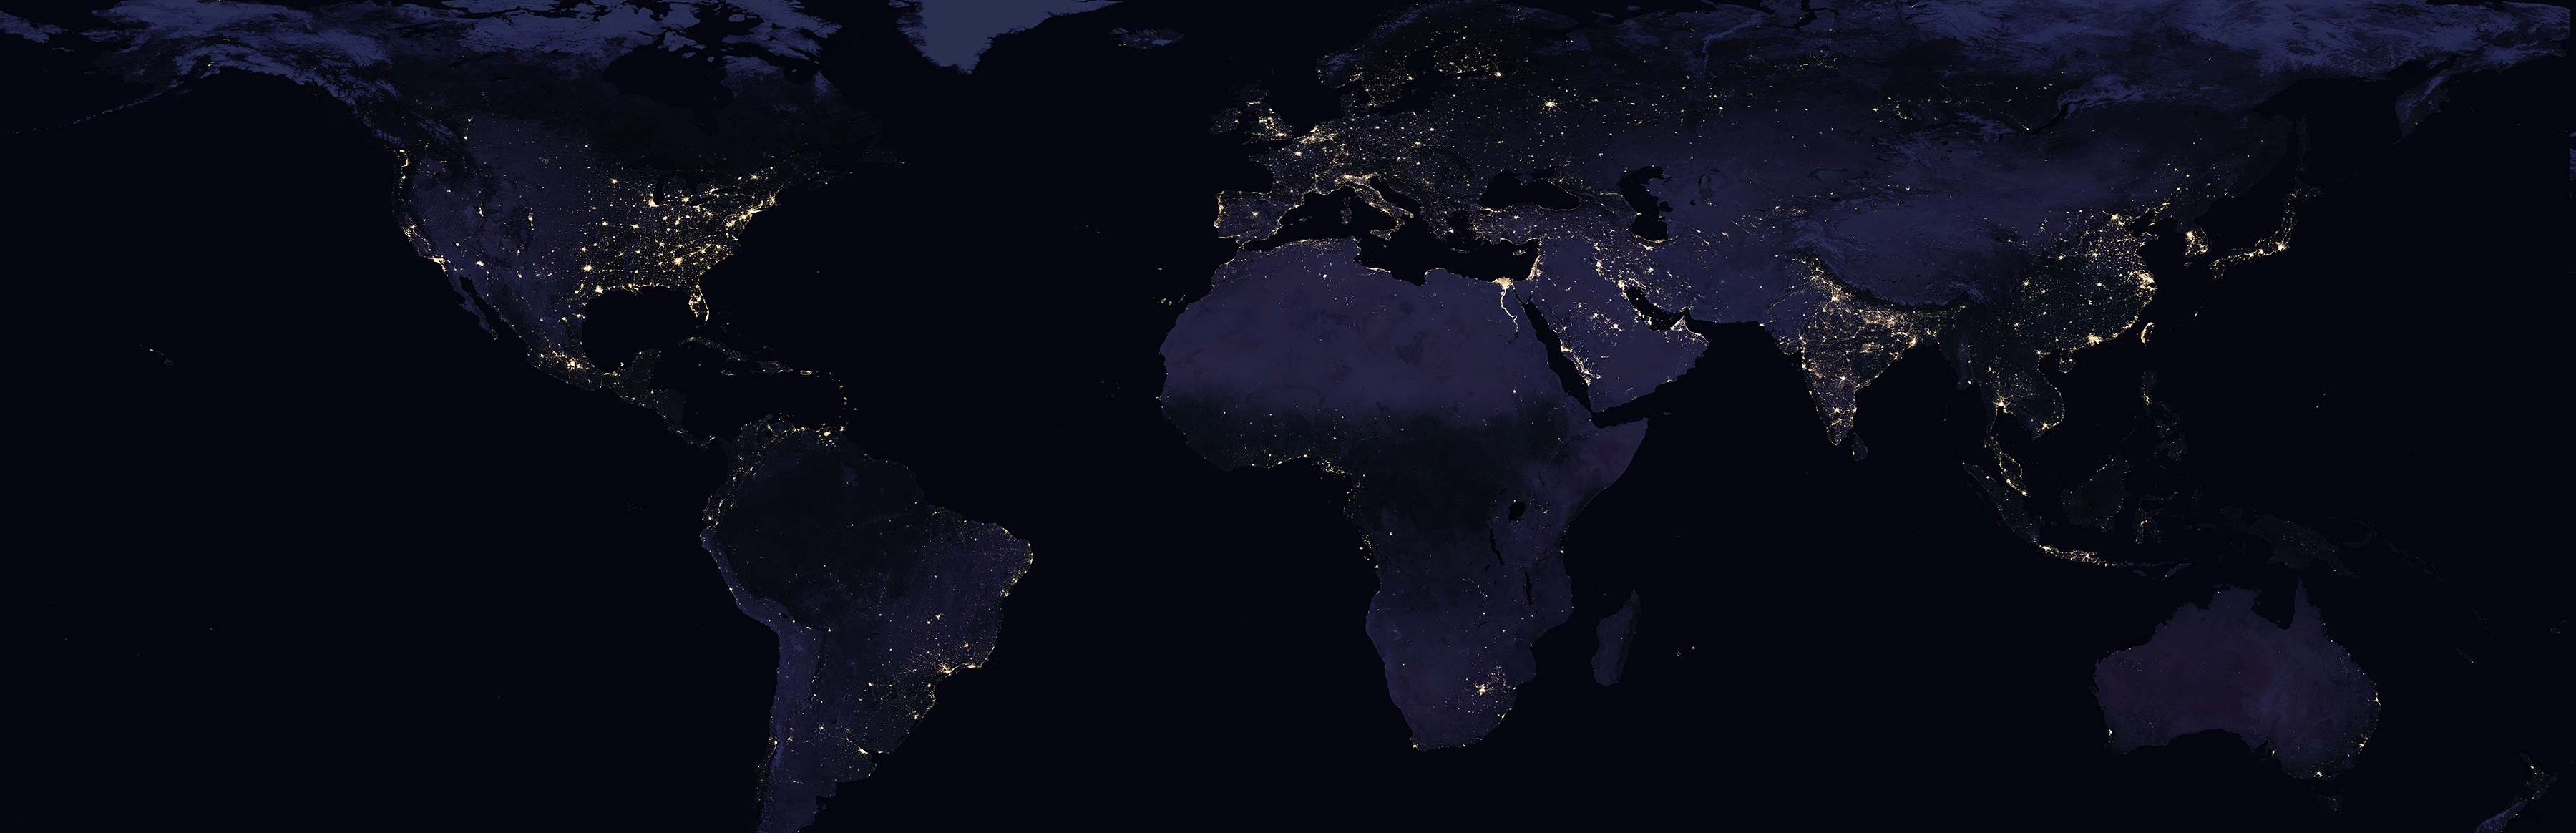
\includegraphics[width = 1.03\textwidth]{img/night-lights-cropped.jpg}
\end{figure}

%\begin{quotation}
%	\noindent``\textit{You can't really know anything if you just remember isolated facts. If the facts don't hang together on a latticework of theory, you don't have them in a usable form. You've got to have models in your head.}''\\
%	\\
%	--Charlie Munger (investor, vice chairman of Berkshire Hathaway)
%\end{quotation}

%% PREAMBLE %%
\onehalfspacing

% Loosely guessed from this: https://www.sciencealert.com/half-the-world-s-population-lives-on-1-of-its-land

\noindent Over half of the Earth's population lives within the sea of city lights visible on the satellite map above. These cities are the centers of global commerce and culture, but in order to function, they require effective governance. Cities need roads, schools, police, fire protection, parks, buses, sewers, and electricity. Many of our most pressing political problems --- including education, criminal justice reform, housing, and climate change --- are in large part problems of city politics.

In this course, we explore how research from political science, economics, sociology, psychology, and mathematics can help us build cities that are healthier, safer, fairer, and more livable for their residents. The semester will be organized around seven themes: the historical origins of cities, political geography, city limits, strengthening local democracy, transportation policy, housing policy, and finally a look at some of the unique challenges facing our community here in Athens, GA. 

%\section*{Course Objectives}
%%\vskip.15in
%%\noindent\textbf{Course Objectives:}  
%By the end of this course, you will be able to:
%\begin{itemize}
%	\item 
%	\item 
%	\item
%\end{itemize}


\section*{Course Structure}

We will meet twice a week on Tuesdays and Thursdays, and each class period will be dedicated to one of the seven themes above (see our \href{https://joeornstein.github.io/pols-4641/}{course website} for a detailed schedule and course readings). During the semester, you will create and publish one Science Communication Project, in which you teach an ``outside'' audience an idea from the course. The format for these projects can be anything except a standard essay. And no Twitter threads. Otherwise, feel free to be creative. The project could be aimed at a social media audience (e.g. Instagram story, TikTok/YouTube video), a policy audience (letter to a public official, presentation at a public meeting), or some other audience (podcast, editorial, blog post, policy brief). Feel free to discuss alternative formats with me. The purpose of these assignments is to get you out of ``writing for your professor'' mode and into a mode where your work has some broader impact on the world.

Every two weeks, we discuss a new theme and begin a new set of projects. The core loop looks something like this. 

\begin{itemize}
	\item \textbf{Day 1 (Thursday): Lecture.} I will introduce this week's theme, and then randomly assign students to teams. Students completing projects will introduce themselves, describe the topics they find most interesting, and leave with a research plan for Journal Club the following week.
	\item \textbf{Day 2 (Tuesday): Journal Club.} Discuss what you learned from the readings. The objective of Journal Club is to help students decide on an idea/audience for their projects, and to leave with an annotated list of citations. 
	\item \textbf{Day 3 (Thursday): Table Read.} Students come to class with a rough draft of their project, and the team suggests edits and helps turn it into a final draft. (Something like a shared Google Doc is useful here.)
	\item \textbf{Day 4 (Tuesday): Symposium.} A mini-conference where students share their projects and answer questions about this week's theme.
\end{itemize}

\noindent The following Thursday, we start the loop over again with a new theme. During the final two weeks of class, students will work together in groups of at most five to deliver a final presentation that addresses an ongoing political issue in Athens, GA. More details on these problems will be available towards the end of the semester. 

\section*{Grading}

Your grade for the course will be based on four components:

\begin{itemize}
	\item \textbf{Reflection Assignments (20\%).} At the end of each class, you will submit (via Google Form) one new idea you learned in class and one lingering question you still have. I will grade these for completion and use the questions to help guide our subsequent class sessions and symposia.
	\item \textbf{Quizzes (6 $\times$ 5\% each).} Following Symposium days, I will post a short multiple choice quiz on eLC, reviewing the ideas we learned over the past two weeks. Complete the quiz before the following Tuesday's lecture.
	\item \textbf{Science Communication Projects (30\% each).} Remember, I want everyone to ACE these projects. They should satisfy the following three criteria, each worth ten points (where 10/10 is perfect, 9/10 contains minor flaws, 8/10 contains multiple flaws, 7/10 contains major flaws, and 6/10 or less means something went terribly wrong):
		\begin{itemize}
			\item \textbf{Accurate (10 points).} These are public-facing projects, so we don't want to be spreading misinformation or half-truths. Make sure that you are clearly and accurately conveying the findings of the scientific research, in a way that your audience would understand and find compelling.
			\item \textbf{Comprehensive (10 points).} This is your one big project of the semester, so you should put in a commensurate amount of effort. Your goal is to convince your audience of a single idea (your \textit{thesis statement}). To that end, you'll need to perform a deep dive into your idea -- deeper than I'm able to go in my lectures -- and cite multiple sources to back up your claims. 
			\item \textbf{Engaging (10 points).} In a world awash with content, 90\% of the battle is grabbing and holding your audience's attention. Humor, stories, and pathos are effective tools for engaging your audience (Memes are nice too.)
		\end{itemize}
	\item \textbf{MVP Awards (10\%).} On Journal Club and Table Read days, you have the opportunity to help your classmates make their projects the best they can be. When students submit their projects, they will be asked to nominate four classmates whose suggestions were the most helpful. You receive 5 percentage points for each MVP nomination you receive, up to a maximum of 10\%. (Note: if everyone is contributing equally, you should expect to receive roughly 4 of these nominations over the course of the semester).
	\item \textbf{Final Presentations (10\%).} Your final presentation should propose a solution to your team's problem that is well-reasoned and reflects a thorough understanding of the course concepts. Exemplary performance on both criteria merits a 10; expect an average grade in the neighborhood of 8-9 points.
\end{itemize}

\noindent Your projects must be published to their intended audience and submitted to eLC 24 hours before your scheduled Symposium. Late projects will receive a full letter grade deduction every 24 hours until they are submitted.

\section*{Office Hours}

I will be available for office hours by appointment, and you can sign up for 20 minute slots through the course website. With each project, you'll simultaneously be learning new content \textit{and} trying to teach others what you've learned. This is a difficult task! I strongly recommend that you sign up for office hours before your project is due so we can discuss any questions you have. Even if you don't have any questions about the material, stop by office hours anyway! One of the great things about college is that your professors are all required to set aside time each week just to talk with their students. And, not to brag, but I'm \textit{pretty good at talking}. My job title (Assistant Professor) is basically just Latin for ``Assistant Talker''.




\section*{Academic Honesty}

Remember that when you joined the University of Georgia community, you agreed to abide by a code of conduct outlined in the academic honesty policy called \href{https://honesty.uga.edu/Academic-Honesty-Policy/Introduction/}{\textit{A Culture of Honesty}}. It has some pretty specific things to say on the subject of cheating. Quite specific. Projects must be your own original creations, and I will report any and all dishonest conduct to the Office of the Vice President for Instruction. If you use a language model such as ChatGPT to generate text or images for your assignments, you must inform the professor and explicitly note which parts of the text were the language model's contribution. Any other use of such software to disguise plagiarized work is considered unauthorized assistance.

\section*{Mental Health and Wellness Resources}

\begin{itemize}
\item If you or someone you know needs assistance, you are encouraged to contact Student Care and Outreach in the Division of Student Affairs at 706-542-7774 or visit \href{https://sco.uga.edu}{https://sco.uga.edu}. They will help you navigate any difficult circumstances you may be facing by connecting you with the appropriate resources or services. 
\item UGA has several resources for a student seeking \href{https://www.uhs.uga.edu/bewelluga/bewelluga}{mental health services} or \href{https://www.uhs.uga.edu/info/emergencies}{crisis support}. 
\item If you need help managing stress anxiety, relationships, etc., please visit \href{https://www.uhs.uga.edu/bewelluga/bewelluga}{BeWellUGA} for a list of FREE workshops, classes, mentoring, and health coaching led by licensed clinicians and health educators in the University Health Center.
\item Additional resources can be accessed through the UGA App.
\end{itemize}



%%%%%% THE END 
\end{document} 